%!TEX root = ../tcc.tex

\chapter{Transmission e o BCC}
\label{chap:bcc}

Neste texto, descrevemos que são encontrados vários elementos de Ciência da Computação
no programa cliente Transmission. A intenção agora é encontrar quais disciplinas da
grade curricular do Bacharelado em Ciência da Computação (BCC) tem conhecimentos
utilizados no Transmission.

\begin{figure}[H]
    \centering
    \fbox{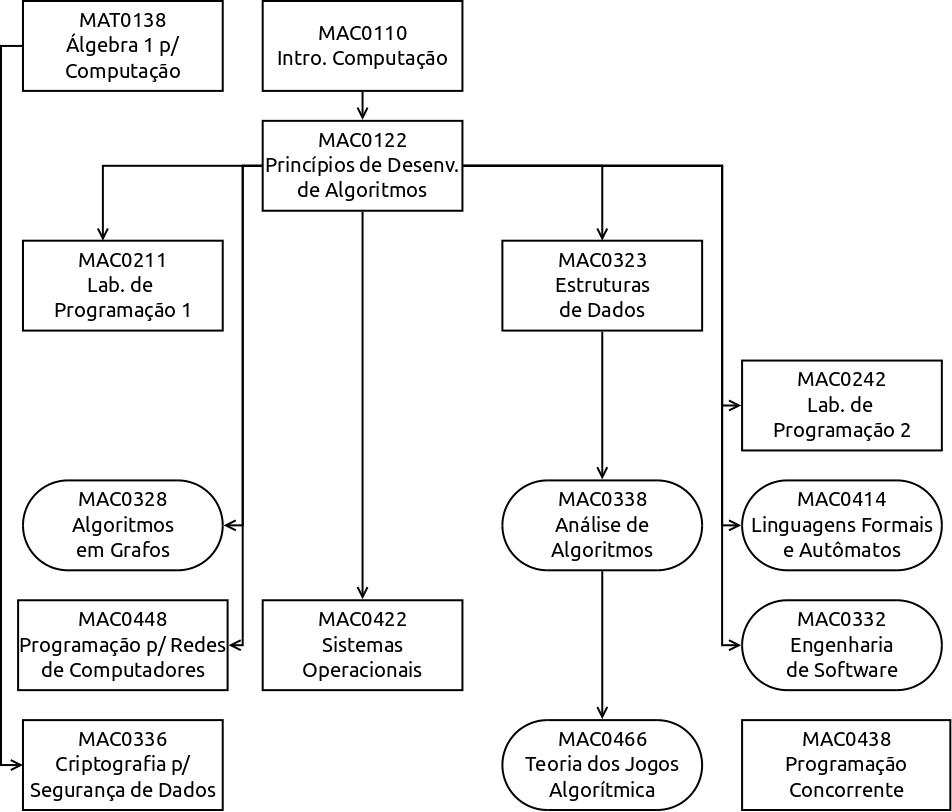
\includegraphics[width=.75\textwidth]{mapa-bcc.png}}
    \caption{disciplinas do BCC utilizadas diretamente na programação do Transmission,
    ligadas pelos seus pré-requisitos. As bordas arredondadas indicam que o
    conhecimento auxilia, mas não é necessário.}
    \label{fig:bcc}
\end{figure}

Das disciplinas do BCC, as reconhecidas como necessárias para o entendimento do
BitTorrent e o Transmission foram:

\begin{itemize}
    \item \textbf{MAC0110 --- Introdução à Computação} \\
        \textbf{MAC0122 --- Princípios de Desenvolvimento de Algoritmos} \\
        linguagem C e algoritmos básicos.

    \item \textbf{MAC0211 --- Laboratórios de Programação 1} \\
        organização de código, trabalho gerenciado em grupos de desenvolvedores,
        controle de versão de código fonte (Git), portabilidade de código entre
        plataformas (Autoconf e Automake), ferramentas de linha de comando UNIX (grep,
        find, sed), documentação (\LaTeX);

    \item \textbf{MAC0242 --- Laboratório de Programação 2} \\
        \textbf{MAC0332 --- Engenharia de Software} \\
        uso de IDE de desenvolvimento (Eclipse), criação de programas complexos,
        uso de bibliotecas (GTK+);

    \item \textbf{MAC0323 --- Estruturas de Dados} \\
        utilização e manipulação de estruturas de dados, como vetores e listas ligadas;

    \item \textbf{MAC0328 --- Algoritmos em Grafos} \\
        entendimento do algoritmo de busca de nós no \gls{dht};

    \item \textbf{MAC0328 --- Análise de Algoritmos} \\
        \textbf{MAC0446 --- Teoria dos Jogos Algorítmica} \\
        algoritmo da troca das partes entre \glspl{peer};

    \item \textbf{MAT0138 --- Álgebra 1} \\
        \textbf{MAC0336 --- Criptografia para Segurança de Dados} \\
        noções de Álgebra modular e seus usos nos métodos criptográficos;

    \item \textbf{MAC0448 --- Programação para Redes} \\
        desenvolvimento de código de conexão via Internet, como \gls{tcp} e \gls{udp},
        multicast, \gls{nat}, IPv6, UPnP e \gls*{nat}-PMP;

    \item \textbf{MAC0414 --- Linguagens Formais e Autômatos} \\
        uso de autômatos para entendimento dos estados que \glspl*{peer} podem assumir
        e suas transições com as trocas de mensagens \cite{conf:swarming}; e

    \item \textbf{MAC0422 --- Sistemas Operacionais} \\
        \textbf{MAC0438 --- Programação Concorrente} \\
        uso de \glspl{thread} e métodos para computação com seus usos, como acesso à
        memória compartilhada (\emph{mutex}) e travas, e entendimento de caches de
        memória na leitura e escrita de dados.
\end{itemize}

\afterpage{\clearpage}